% !TeX program = pdfLaTeX
\documentclass[smallextended]{svjour3}       % onecolumn (second format)
%\documentclass[twocolumn]{svjour3}          % twocolumn
%
\smartqed  % flush right qed marks, e.g. at end of proof
%
\usepackage{amsmath}
\usepackage{graphicx}
\usepackage[utf8]{inputenc}

\usepackage[hyphens]{url} % not crucial - just used below for the URL
\usepackage{hyperref}

%
% \usepackage{mathptmx}      % use Times fonts if available on your TeX system
%
% insert here the call for the packages your document requires
%\usepackage{latexsym}
% etc.
%
% please place your own definitions here and don't use \def but
% \newcommand{}{}
%
% Insert the name of "your journal" with
% \journalname{myjournal}
%

%% load any required packages here
\usepackage{subcaption} \usepackage{bm} \usepackage{bbm} \usepackage{color} \DeclareMathOperator{\var}{{var}} \DeclareMathOperator{\cov}{{cov}}


% tightlist command for lists without linebreak
\providecommand{\tightlist}{%
  \setlength{\itemsep}{0pt}\setlength{\parskip}{0pt}}


% Pandoc citation processing
\newlength{\cslhangindent}
\setlength{\cslhangindent}{1.5em}
\newlength{\csllabelwidth}
\setlength{\csllabelwidth}{3em}
\newlength{\cslentryspacingunit} % times entry-spacing
\setlength{\cslentryspacingunit}{\parskip}
% for Pandoc 2.8 to 2.10.1
\newenvironment{cslreferences}%
  {}%
  {\par}
% For Pandoc 2.11+
\newenvironment{CSLReferences}[2] % #1 hanging-ident, #2 entry spacing
 {% don't indent paragraphs
  \setlength{\parindent}{0pt}
  % turn on hanging indent if param 1 is 1
  \ifodd #1
  \let\oldpar\par
  \def\par{\hangindent=\cslhangindent\oldpar}
  \fi
  % set entry spacing
  \setlength{\parskip}{#2\cslentryspacingunit}
 }%
 {}
\usepackage{calc}
\newcommand{\CSLBlock}[1]{#1\hfill\break}
\newcommand{\CSLLeftMargin}[1]{\parbox[t]{\csllabelwidth}{#1}}
\newcommand{\CSLRightInline}[1]{\parbox[t]{\linewidth - \csllabelwidth}{#1}\break}
\newcommand{\CSLIndent}[1]{\hspace{\cslhangindent}#1}

\usepackage{hyperref}
\usepackage[utf8]{inputenc}
\def\tightlist{}
\usepackage{lineno}
\linenumbers

\usepackage{booktabs}
\usepackage{longtable}
\usepackage{array}
\usepackage{multirow}
\usepackage{wrapfig}
\usepackage{float}
\usepackage{colortbl}
\usepackage{pdflscape}
\usepackage{tabu}
\usepackage{threeparttable}
\usepackage{threeparttablex}
\usepackage[normalem]{ulem}
\usepackage{makecell}
\usepackage{xcolor}
\begin{document}


\title{An Application of Spatio-temporal Modeling to Finite Population
Abundance Prediction }


    \titlerunning{Spatio-temporal Prediction for Finite Populations}

\author{  }


\institute{
    }

\date{Received: date / Accepted: date}
% The correct dates will be entered by the editor


\maketitle

\begin{abstract}
Spatio-temporal models can be used to analyze data collected at various
spatial locations throughout multiple time points. However, even with a
finite number of spatial locations, there may be a lack of resources to
collect data from every spatial location at every time point. We develop
a spatio-temporal finite-population block kriging (ST-FPBK) method to
predict a quantity of interest, such as a mean or total, across a finite
number of spatial locations. This ST-FPBK predictor incorporates an
appropriate variance reduction for sampling from a finite population.
Through an application to moose surveys in the east-central region of
Alaska, we show that the predictor has a substantially smaller standard
error compared to a predictor from the purely spatial model that is
currently used to analyze moose surveys in the region. We also show how
the model can be used to forecast a prediction for abundance in a time
point for which spatial locations have not yet been surveyed. A separate
simulation study shows that the spatio-temporal predictor is unbiased
and that prediction intervals from the ST-FPBK predictor attain
appropriate coverage. For ecological monitoring surveys completed with
some regularity through time, use of ST-FPBK could improve precision. We
also give an \texttt{R} package that ecologists and resource managers
could use to incorporate data from past surveys in predicting a quantity
from a current survey.
\\
\keywords{
        forecast; kriging; resource monitoring; spatial; temporal;
total \and
    }


\end{abstract}


\def\spacingset#1{\renewcommand{\baselinestretch}%
{#1}\small\normalsize} \spacingset{1}


\hypertarget{intro}{%
\section{Introduction}\label{intro}}

\hypertarget{background}{%
\subsection{Background}\label{background}}

Spatio-temporal data are indexed by both a spatial index, which we will
refer to as a ``site,'' and by a temporal index, which we will refer to
as a ``time point.'' Common examples of spatio-temporal data include
infections from a disease in a country or region collected over a time
period (e.g. Martínez-Beneito, López-Quilez, and Botella-Rocamora 2008;
Sahu and Böhning 2022) or climate variables that are recorded through
time at multiple locations (Lemos and Sansó 2009). Models for
spatio-temporal data have applications in a wide variety of scientific
fields (Cressie and Wikle 2015; Wikle, Zammit-Mangion, and Cressie 2019;
Porcu, Furrer, and Nychka 2021).

One such application is ecological monitoring of a particular resource,
such as animal or plant counts, rainfall, concentration of a compound in
soil samples, etc. A common goal of ecological monitoring is to predict
the total abundance of a resource at the most recent time point using
data collected in subsets of the region at multiple time points. Often,
the region of interest is divided into a finite number of areal sampling
units and data is collected everywhere within a subset of these areal
sampling units at each time point. The remaining areal units are then
left unsampled. We refer to the goal of predicting abundance in the most
recent time point as \emph{spatio-temporal abundance prediction}.

Classical sampling techniques can be used for spatio-temporal abundance
prediction: inference in classical sampling is based on the mechanism in
which units are randomly selected to be in the sample. For example, Wang
and Zhu (2019) use a spatio-temporally balanced sampling design to
construct estimators for finite quantities, like abundance. Panel
sampling designs can also be used when data are sampled over multiple
time points (Urquhart 2012). However, model-assisted techniques and
purely model-based techniques can provide increased precision in
predicting finite quantities, at the cost of placing additional
assumptions on the model generating the observed data (Breidt and
Opsomer 2017; Dumelle et al. 2022).

A few common ways to formally model spatio-temporal covariance include
the product model, the sum model, and the product-sum model. If we
consider \(\text{Cov}(\mathbf{h}_s, h_t)\) to be the covariance between
two data points with spatial separation \(\mathbf{h}_s\) and temporal
separation \(h_t\), then a product model for this covariance (also known
as a ``separable'' model) is
\(\text{Cov}_s(\mathbf{h}_s) \text{Cov}_t(h_t)\), where
\(\text{Cov}_s(\mathbf{h}_s)\) only depends on the spatial separation
and \(\text{Cov}_t(h_t)\) only depends on the temporal separation (Posa
1993; Stein 2005). On the other hand, a sum model for
\(\text{Cov}(\mathbf{h}_s, h_t)\) adds together the spatial and temporal
covariance as \(\text{Cov}_s(\mathbf{h}_s) + \text{Cov}_t(h_t)\)
(Rouhani and Hall 1989). A product-sum model combines the product model
and the sum model: \mbox{} \begin{equation}
\text{Cov}(\mathbf{h}_s, h_t) = w_1\text{Cov}_s(\mathbf{h}_s) \text{Cov}_t(h_t) + w_2\text{Cov}_s(\mathbf{h}_s) + w_3\text{Cov}_t(h_t),
\end{equation}

\noindent where \(w_1\), \(w_2\), and \(w_3\) are non-negative weights
(De Cesare, Myers, and Posa 2001; S. De Iaco, Myers, and Posa 2002). In
general, the product-sum model is more flexible than the product model
and the sum model. Chen, Genton, and Sun (2021) provide a general review
for modeling spatio-temporal data.

These spatio-temporal models can be used for abundance prediction in a
Bayesian framework as well as in a frequentist framework. Within the
Bayesian framework, spatio-temporal modeling is often used as part of a
hierarchical model for the response variable: Conn et al. (2015) offer a
review of such methods as well as issues with using spatio-temporal
modeling for abundance prediction for a few different hierarchical model
structures. Bayesian hierarchical models have been used for
spatio-temporal abundance prediction by Ver Hoef and Jansen (2007) for
harbor seals in Alaska, Sauer and Link (2011) for birds in North
America, Davy, Squires, and Zimmerling (2021) for bats in Canada, Adde
et al. (2020) for waterfowl in Canada, and Schmidt et al. (2022) for
moose in Alaska. Additionally, Ross, Hooten, and Koons (2012) use
Integrated Nested Laplace Approximation (INLA) to model spatio-temporal
abundance data in a hierarchical framework. While a Bayesian
hierarchical models allow for a large amount of flexibility in the model
formulation and are thus powerful tools for statistical inference, Conn
et al. (2015) note that ``care must be taken to tailor models to match
the study population and survey data available.'' We discuss Bayesian
hierarchical models for abundance prediction more in Section
\ref{section:Discussion}.

Spatio-temporal predictions can also be constructed in a frequentist
framework. As a couple of recent examples, Breivik et al. (2021) use a
Gaussian model to predict abundance of cod in the Barents Sea, and Stock
et al. (2020) use random forests, generalized additive models, and
Gaussian Markov random fields to predict bycatch of a few species of
fish. While a prediction for the total abundance is fairly
straightforward to obtain in the frequentist setting (by making
predictions for the response at each unobserved site and then summing
the observed response values with the predictions), obtaining the
prediction variance is more challenging. If the number of sites in the
region of interest is finite, then the spatio-temporal abundance
prediction variance should incorporate a finite population correction
such that, if all spatial sites are sampled in the most recent time
point, the prediction variance for the total abundance in the most
recent time point is equal to 0.

Our primary goal in this paper is to develop such a
finite-population-prediction-variance correction. We extend the work of
Ver Hoef (2008), who developed Finite Population Block Kriging (FPBK) to
predict a linear function of the realized values of a response variable
(such as the total abundance) for a survey at one particular time point,
incorporating a finite population correction to the variance of the
predictor. In this paper, we broaden the approach of Ver Hoef (2008) to
the spatio-temporal context, appropriately adjusting the
finite-population-prediction-variance correction and allowing for the
covariance matrix of the response vector to include spatio-temporal
structure.

\hypertarget{motivating-example}{%
\subsection{Motivating Example}\label{motivating-example}}

To motivate the development of the predictor in Section
\ref{section:Methods}, we consider moose surveys, which are performed
annually or every other year in many regions of Alaska and western
Canada. The most common goal of these surveys is to predict moose
abundance, the total number of moose, in some finite region to inform
harvest regulations (Kellie, Colson, and Reynolds 2019). The region of
interest is divided into a finite number of areal polygons. Because of
time and money constraints, only some polygons, or sites, in the region
of interest are selected to be in the survey at a particular time point.
Biologists fly to these selected sites, count the number of moose, and
then use FPBK to find a prediction for the abundance for that year. Note
that the interest is in predicting the realized total abundance so that,
if there were enough resources to survey every site in a year, we would
know the abundance in that year exactly. These surveys are historically
analyzed with the ``WinfoNet'' site developed by DeLong (2006), which
calculates the ``GeoSpatial Population Estimator'' (GSPE) for a given
survey. The GSPE is an application of the FPBK predictor developed by
Ver Hoef (2008).

Though many of these surveys are completed regularly, most are analyzed
completely independently of surveys from previous years (e.g. Gasaway et
al. 1986; Kellie and DeLong 2006; Boertje et al. 2009; Peters et al.
2014). For example, a model for a survey conducted in the year 2019
constructs a prediction for total abundance only from counts on sites
that were sampled in that year. However, using counts from previous
years in a model that incorporates both spatial and temporal
(spatio-temporal) correlation while also using a finite population
correction factor based on the proportion of sites surveyed in the most
recent year could result in a prediction for the realized total that is
more precise than predictions from a purely spatial model. Shortly, we
describe such a predictor.

The rest of this paper is organized as follows. In Section
\ref{section:Methods}, we couple spatio-temporal modeling with finite
population prediction to develop the Best-Linear-Unbiased-Predictor
(BLUP) and its prediction variance for any linear function of a general
response variable, including the total abundance across all sites at a
particular time point. We call this predictor the ST-FPBK
(spatio-temporal Finite Population Block Kriging) predictor. In Section
\ref{section:Application}, we apply ST-FPBK to a moose data set in the
east-central region of Alaska. In Section \ref{section:Simulation}, we
conduct a simulation study to examine the properties of the ST-FPBK
predictor and compare its performance to a predictor from a purely
spatial model and a simple random sample design-based estimator.
Finally, in Section \ref{section:Discussion}, we offer additional
thoughts on the application and simulation, and we give directions for
future research.

\hypertarget{section:Methods}{%
\section{Methods}\label{section:Methods}}

We now give details on the development of the spatio-temporal model and
subsequently use this model to extend the approach of Ver Hoef (2008),
developing a finite population correction factor to give a
Best-Linear-Unbiased-Predictor (BLUP) and its prediction variance for
any linear function of the response vector.

\hypertarget{spatio-temporal-model}{%
\subsection{Spatio-temporal Model}\label{spatio-temporal-model}}

Let \(Y(\mathbf{s}_{i}, t_j)\), \(i = 1, 2, \ldots, n_{s}\) and
\(j = 1, 2, \ldots, n_{t}\), be a random variable indexed by a spatial
site and a time point, where the vector \(\mathbf{s}_i\) contains the
coordinates for the \(i^{th}\) spatial site, \(n_s\) is the number of
unique sites, \(t_j\) is the time index for the \(j^{th}\) time point,
and \(n_t\) is the number of unique time points. If each site is
represented at every time point, a vector of the
\(Y(\mathbf{s}_{i}, t_j)\), denoted \(\mathbf{y}\), has length
\(n_{s} \cdot n_{t} \equiv N\). Then, a spatio-temporal model for
\(\mathbf{y}\) is \mbox{} \begin{equation}
\mathbf{y} = \mathbf{X} \bm{\beta} + \bm{\epsilon},
\end{equation}

\noindent where \(\mathbf{X}\) is a design matrix for the fixed effects
and \(\bm{\beta}\) is a parameter vector of fixed effects. As in Dumelle
et al. (2021), we can decompose the error vector \(\bm{\epsilon}\) into
spatial, temporal, and spatio-temporal components, each of which will be
explained in detail in the subsequent paragraphs: \mbox{}
\begin{equation} \label{equation:basicmod}
\bm{\epsilon} = \mathbf{Z}_{s} \bm{\delta} + \mathbf{Z}_{s} \bm{\gamma} + \mathbf{Z}_t \bm{\tau} + \mathbf{Z}_t \bm{\eta} + \bm{\omega} + \bm{\nu}.
\end{equation}

In the spatial component of equation \ref{equation:basicmod}
(\(\mathbf{Z}_{s} \bm{\delta} + \mathbf{Z}_{s} \bm{\gamma}\)), the
matrix \(\mathbf{Z}_{s}\) is an \(N \times n_s\) matrix of \(0\)'s and
\(1\)'s, where the values in a row corresponding to a data point at site
\(\mathbf{s}_{i}\) are \(1\) in the \(i^{th}\) column and \(0\) in all
other columns. \(\bm{\delta}\) is a random vector with mean
\(\mathbf{0}\) and covariance
\(\mathop{\mathrm{{cov}}}(\bm{\delta}) = \sigma^2_{\delta} \mathbf{R}_{s}\),
where \(\mathbf{R}_s\) is an \(n_s \times n_s\) spatial correlation
matrix and \(\sigma^2_{\delta}\) is called the spatial dependent error
variance (or spatial partial sill). The random vector \(\bm{\gamma}\)
also has mean \(\mathbf{0}\) but has covariance
\(\mathop{\mathrm{{cov}}}(\bm{\gamma}) = \sigma^2_{\gamma} \mathbf{I}_{s}\),
where \(\mathbf{I}_s\) is the \(n_s \times n_s\) identity matrix and
\(\sigma^2_{\gamma}\) is called the spatial independent error variance
(or spatial nugget).

In the temporal component of equation \ref{equation:basicmod}
(\(\mathbf{Z}_t \bm{\tau} + \mathbf{Z}_t \bm{\eta}\)),
\(\mathbf{Z}_{t}\) is an \(N \times n_t\) matrix of \(0\)'s and \(1\)'s,
where the values in a row corresponding to a data point at time point
\(t_j\) are \(1\) in the \(j^{th}\) column and \(0\) in all other
columns. \(\bm{\tau}\) is a random vector with mean \(\mathbf{0}\) and
covariance
\(\mathop{\mathrm{{cov}}}(\bm{\tau}) = \sigma^2_{\tau} \mathbf{R}_{t}\),
where \(\mathbf{R}_t\) is an \(n_t \times n_t\) temporal correlation
matrix and \(\sigma^2_{\tau}\) is called the temporal dependent error
variance (or temporal partial sill). \(\bm{\eta}\) is also a random
vector with mean \(\mathbf{0}\) but has covariance
\(\mathop{\mathrm{{cov}}}(\bm{\eta}) = \sigma^2_{\eta} \mathbf{I}_{t}\),
where \(\mathbf{I}_t\) is the \(n_t \times n_t\) identity matrix and
\(\sigma^2_{\eta}\) is called the temporal independent error variance
(or temporal nugget).

In the spatio-temporal component of equation \ref{equation:basicmod}
(\(\bm{\omega} + \bm{\nu}\)), \(\bm{\omega}\) is a random vector with
mean \(\mathbf{0}\) and covariance
\(\mathop{\mathrm{{cov}}}(\bm{\omega}) = \sigma^2_{\omega} \mathbf{R}_{st}\),
where \(\mathbf{R}_{st}\) is an \(N \times N\) spatio-temporal
correlation matrix and \(\sigma^2_{\omega}\) is sometimes called the
spatio-temporal dependent error variance (or spatio-temporal partial
sill). \(\bm{\nu}\) is also a random vector with mean \(\mathbf{0}\) but
has covariance
\(\mathop{\mathrm{{cov}}}(\bm{\nu}) = \sigma^2_{\nu} \mathbf{I}_{st}\),
where \(\mathbf{I}_{st}\) is the \(N \times N\) identity matrix and
\(\sigma^2_{\nu}\) is sometimes called the spatio-temporal independent
error variance (or spatio-temporal nugget).

Though there are a few types of models for the errors that can be built
from equation \ref{equation:basicmod} by setting certain error variances
to 0 (e.g.~a sum-with-error model sets \(\sigma^2_{\omega} = 0\)) and/or
by allowing \(\mathbf{R}_{st}\) to take certain forms (e.g.~a separable
model sets all covariance parameters equal to \(0\) except
\(\sigma^2_{\omega}\) and uses the structure for \(\mathbf{R}_{st}\)
given in equation \ref{equation:Rst} below), we focus only on the
product-sum model (De Cesare, Myers, and Posa 2001; Sandra De Iaco,
Myers, and Posa 2001). In a common formulation of the product-sum model,
\(\mathbf{R}_{st}\) is \mbox{} \begin{equation}
\label{equation:Rst}
\mathbf{R}_{st} \equiv \mathbf{Z}_{s} \mathbf{R}_{s} \mathbf{Z}_{s}' \odot \mathbf{Z}_t \mathbf{R}_t \mathbf{Z}_t',
\end{equation} \noindent where \(\odot\) is the Hadamard product
operator. Note that, in order to save on the number of parameters, we
will assume that the \(\mathbf{R}_s\) and \(\mathbf{R}_t\) that form
\(\mathbf{R}_{st}\) are the same as the \(\mathbf{R}_s\) and
\(\mathbf{R}_t\) associated with \(\bm{\delta}\) and \(\bm{\tau}\),
respectively, although this is not necessary in general.
\(\mathbf{R}_s\) can be parameterized in different ways, but one common
assumption is to assume the covariance function generating
\(\mathbf{R}_s\) is second-order stationary (ie. the covariance between
two data points is a function only of the separation vector between two
sites) and isotropic (ie. the covariance is a function of the distance
only and does not depend on the direction of the separation vector). For
example, the exponential covariance function is defined as follows. For
observations at sites \(i\) and \(i'\) at \(h_{ii'}\) distance apart,
row \(i\) and column \(i'\) of \(\mathbf{R}_{s}\) is equal to \mbox{}
\begin{equation}
\label{equation:spatcov}
\text{exp}(-h_{ii'} / \phi),
\end{equation} \noindent where \(\text{exp}(x)\) is equivalent to
\(e^x\) and \(\phi\) is a spatial range parameter controlling the decay
rate of the covariance as distance between two sites increases (Cressie
2015).

Similarly, one common assumption when parameterizing \(\mathbf{R}_t\) is
to assume the covariance function generating \(\mathbf{R}_t\) is
second-order stationary (ie. the covariance is a function only of the
temporal distance). For example, the exponential covariance function is
defined as follows. For observations at time points \(j\) and \(j'\) at
\(m_{jj'}\) units apart, row \(j\) and column \(j'\) of
\(\mathbf{R}_{t}\) is equal to \mbox{} \begin{equation}
\label{equation:tempcov}
\text{exp}(-m_{jj'} / \rho),
\end{equation} \noindent where \(\rho\) is a temporal range parameter
controlling the decay rate of the covariance as the number of time units
between two data points increases. Note that the exponential form of
\(\mathbf{R}_t\) is equivalent to an AR(1) time series model if the time
points are equally spaced and the correlation parameter in the AR(1)
series is greater than zero (Schabenberger and Gotway 2017).

The product-sum model for \(\mathbf{y}\) is then \mbox{}
\begin{equation} \label{equation:model}
\mathbf{y} = \mathbf{X} \bm{\beta} + \mathbf{Z}_{s} \bm{\delta} + \mathbf{Z}_{s} \bm{\gamma} + \mathbf{Z}_t \bm{\tau} + \mathbf{Z}_t \bm{\eta} + \bm{\omega} + \bm{\nu},
\end{equation}

\noindent where \(\bm{\delta}\), \(\bm{\gamma}\), \(\bm{\tau}\),
\(\bm{\eta}\), \(\bm{\omega}\), and \(\bm{\nu}\) are mutually
independent, \(\mathbf{y}\) has mean \(\mathbf{X} \bm{\beta}\), and
\(\mathbf{y}\) has covariance \mbox{} \begin{equation}
\label{equation:var}
\mathop{\mathrm{{var}}}(\mathbf{y}) \equiv \bm{\Sigma} = \sigma^2_{\delta} \mathbf{Z}_{s} \mathbf{R}_{s} \mathbf{Z}_{s}' + \sigma^2_{\gamma} \mathbf{Z}_{s} \mathbf{I}_{s} \mathbf{Z}_{s}' + \sigma^2_{\tau} \mathbf{Z}_t \mathbf{R}_t \mathbf{Z}_t'+ \sigma^2_{\eta} \mathbf{Z}_t \mathbf{I}_t \mathbf{Z}_t' + \sigma^2_{\omega} \mathbf{R}_{st} + \sigma^2_{\nu} \mathbf{I}_{st}.
\end{equation}

\noindent There are a few reasons why we choose to solely focus on the
product-sum model. First, as long as \(\mathbf{R}_s\) and
\(\mathbf{R}_t\) are positive definite and either
\(\sigma^2_{\omega} > 0\) or \(\sigma^2_{\nu} > 0\), then the covariance
matrix in equation \ref{equation:var} is also positive definite (De
Cesare, Myers, and Posa 2001; Sandra De Iaco, Myers, and Posa 2001).
Also, the product-sum model is non-separable, giving it more flexibility
than a separable (product) model for the covariance (S. De Iaco, Palma,
and Posa 2015; Dumelle et al. 2021). Xu and Shu (2015) claim that the
product-sum model is the most widely used spatio-temporal model used in
practical applications.

\hypertarget{subsection:fpbk}{%
\subsection{Finite Population Block Kriging}\label{subsection:fpbk}}

The model that we developed in the previous section in equation
\ref{equation:model} is for the \(N\)-length vector \(\mathbf{y}\).
However, often we do not have the resources to sample or observe every
spatial site during every time point. Therefore, we may have an interest
in prediction of the response values on sites that were not observed,
particularly sites in the most recent time point. Throughout this
section, let the subscript \(o\) denote data points that were
``observed'' or sampled, the subscript \(u\) denote data points that
were ``unobserved'' or not sampled, and the subscript \(a\) denote
``all'' data points. Then, we can re-order the response vector
\(\mathbf{y}\) so that \mbox{} \begin{equation} \label{equation:ordered}
\mathbf{y} \equiv \mathbf{y}_a = [\mathbf{y}_u', \mathbf{y}_o']'.
\end{equation}

Our primary goal is to use the model developed for \(\mathbf{y}_a\) in
equation \ref{equation:model} to find optimal weights \(\mathbf{q}'\) to
apply to the observed realizations of \(\mathbf{y}_o\) such that
\(\mathbf{q}' \mathbf{y}_o\) is the Best Linear Unbiased Predictor
(BLUP) for \(\mathbf{b}_a' \mathbf{y}_a\), a linear function of
\(\mathbf{y}_a\). The \(N\)-length vector \(\mathbf{b}_a'\) might be,
for example, a vector of \(1\)'s, in which case we would be predicting
the total response across all sites and all time points. More typical
would be the case where \(\mathbf{b}_a\) has \(1\)'s for all sites in
the current time point and all other elements are \(0\), in which case
we would be predicting the total response in the current time point.

Unbiasedness implies that
\(E(\mathbf{q'}\mathbf{y}_o) = E(\mathbf{b}_a'\mathbf{y}_a)\) for all
\(\bm{\beta}\). So, denoting \(\mathbf{X}_o\) as the \(n_o \times p\)
design matrix for the observed data points (where \(p\) is the number of
fixed effects) and \(\mathbf{X}_a\) as the design matrix for all data
points, \(\mathbf{q'} \mathbf{X}_o \bm{\beta}\) =
\(\mathbf{b'}_a \mathbf{X}_a \bm{\beta}\) for every \(\bm{\beta}\),
implying that \(\mathbf{q'} \mathbf{X}_o = \mathbf{b'}_a \mathbf{X}_a\).
Kriging weights are then found by finding \(\bm{\lambda}_o\), an
\(n_o \times 1\) column vector, where \(n_o\) is the number of observed
data points, such that \mbox{} \begin{equation}
E\{(\mathbf{q'}\mathbf{y}_o - \mathbf{b'}_a \mathbf{y}_a)^2\} - E\{(\bm{\lambda}_o'\mathbf{y}_o - \mathbf{b'}_a \mathbf{y}_a)^2\}
\end{equation} \noindent is greater than 0 for all \(\mathbf{q'}\). The
prediction equations are

\begin{equation}
\begin{pmatrix}
\bm{\Sigma}_{o, o} & \mathbf{X}_o \\
\mathbf{X}_o' & \mathbf{0}
\end{pmatrix} 
\begin{pmatrix}
\bm{\lambda} \\
\mathbf{m}
\end{pmatrix} = 
\begin{pmatrix}
\bm{\Sigma}_{o, o} & \bm{\Sigma}_{o, u} \\
\mathbf{X}_{o}' & \mathbf{X}_{u}'
\end{pmatrix} 
\begin{pmatrix}
\mathbf{b}_{o} \\
\mathbf{b}_{u}
\end{pmatrix},
\end{equation} \noindent where \(\mathbf{m}\) is a \(p\)-length column
vector of the Lagrange multipliers due to the unbiasedness constraint
and the subscripts \(o\) and \(u\) denote observed and unobserved data
points. For example, \(\bm{\Sigma}_{o, o}\) denotes the
\(n_o \times n_o\) submatrix of \(\bm{\Sigma}\) (from equation
\ref{equation:var}) corresponding only to rows and columns of observed
data points and \(\bm{\Sigma}_{u, o}\) denotes the
\((N - n_o) \times n_o\) submatrix of \(\bm{\Sigma}\) corresponding to
rows of data points that were not observed and columns of data points
that were observed. Solving the prediction equations, the optimal
prediction weights that are both unbiased and have the smallest possible
prediction variance compared to any other linear predictor are \mbox{}
\begin{equation}
\bm{\lambda}_o' = \mathbf{b}_{o}' + \mathbf{b}_{u}'\left[ (\bm{\Sigma}_{u, o}\bm{\Sigma}_{o, o}^{-1}) - (\bm{\Sigma}_{u, o} \bm{\Sigma}_{o, o}^{-1})\mathbf{X}_o\mathbf{W}_o^{-1}\mathbf{X}_o'\bm{\Sigma}_{o, o}^{-1} + \mathbf{X}_{u}'\mathbf{W}_o^{-1}\mathbf{X}_o \bm{\Sigma}_{o, o}^{-1} \right],
\end{equation} \noindent where
\(\mathbf{W}_o = \mathbf{X}_o'\bm{\Sigma}_{o, o}^{-1}\mathbf{X}_o\). The
BLUP for \(\mathbf{b}'_a \mathbf{y}_a\) is then \mbox{}
\begin{equation} \label{equation:blup}
\widehat{\mathbf{b}'_a \mathbf{y}_a} = \bm{\lambda}_o' \mathbf{y}_o,
\end{equation} \noindent which is equivalent to \mbox{}
\begin{equation*}
\mathbf{b}_{o}'\mathbf{y}_{o} + \mathbf{b}_{u}' \mathbf{\hat{y}}_{u},
\end{equation*} \noindent where
\(\mathbf{\hat{y}}_{u} = \bm{\Sigma}_{u, o} \Sigma_{o, o}^{-1} (\mathbf{y}_o - \bm{\hat{\mu}}_o) + \bm{\hat{\mu}}_u\)
with \(\bm{\hat{\mu}}_o = \mathbf{X}_o \bm{\hat{\beta}}\) and
\(\bm{\hat{\mu}}_u = \mathbf{X}_u \bm{\hat{\beta}}\).
\(\bm{\hat{\beta}}\) is the generalized least squares estimator
\((\mathbf{X}_o' \bm{\Sigma}_{o, o}^{-1} \mathbf{X}_o)^{-1} \mathbf{X}_o' \bm{\Sigma}_{o, o}^{-1} \mathbf{y}_o\).
We can see then that the predictor multiplies the observed data
\(\mathbf{y}_o\) with relevant weights from the \(\mathbf{b}_o\) vector,
and then adds in the kriged predictions \(\mathbf{\hat{y}}_{u}\)
multiplied with relevant weights from the \(\mathbf{b}_u\) vector.

The finite-population-corrected- variance of the BLUP in equation
\ref{equation:blup} is \mbox{} \begin{equation} \label{equation:predvar}
E((\bm{\lambda}_o'\mathbf{y}_o - \mathbf{b}_a'\mathbf{y}_a)^2) = \\
\bm{\lambda}_o'\bm{\Sigma}_{o, o}\bm{\lambda}_o - 2 \mathbf{b}_a' \bm{\Sigma}_{a, o} \bm{\lambda}_o + \mathbf{b}_a' \bm{\Sigma}_{a, a} \mathbf{b}_a.
\end{equation}

\noindent We call the predictor in equation \ref{equation:blup} with
\(\bm{\Sigma}\) in equation \ref{equation:var} the ST-FPBK predictor.

A common predictor of interest is the total abundance in the most
current time point of the survey. In this scenario, \(\mathbf{b}_a\) is
a vector of \(1\)'s and \(0\)'s, where the \(k^{th}\) element of
\(\mathbf{b}_a\) is equal to \(1\) if the \(k^{th}\) element of
\(\mathbf{y}_a\) is from the most recent time point of the survey and
the \(k^{th}\) element of \(\mathbf{b}_a\) is equal to 0 otherwise. If
we order \(\mathbf{y}_a\) by (1) the unobserved data points from past
surveys, (2) the unobserved data points from the current survey, (3) the
observed data points from past surveys, and (4) the observed data points
from the current survey, then \mbox{}
\begin{equation} \label{equation:currentweights}
\mathbf{b}_a = [\mathbf{b}_{up}', \mathbf{b}_{uc}', \mathbf{b}_{op}', \mathbf{b}_{oc}']' = [\mathbf{0}', \mathbf{1}', \mathbf{0}', \mathbf{1}']',
\end{equation} \noindent where the subscripts \(up\), \(uc\), \(op\),
and \(oc\) denote unobserved sites in past surveys, unobserved sites in
the current survey, observed sites in past surveys, and observed sites
in the current survey, respectively.

Though we are interested in predicting \(\mathbf{b}_a ' \mathbf{y}_a\)
in the development above so that we are predicting a single quantity of
interest and obtaining a single finite-population-corrected-prediction
variance, we can also predict for multiple quantities of interest and
obtain a prediction covariance matrix with \(\mathbf{B}' \mathbf{y}_a\),
where \(\mathbf{B}\) is an \(N \times n_{pred}\) matrix and \(n_{pred}\)
is the number of different quantities we wish to predict. One setting
where such development is potentially useful is predicting the total
abundance for each time point in the study, as is done in Section
\ref{section:Application} in Figure \ref{fig:trend}.

\hypertarget{estimation}{%
\subsection{Estimation}\label{estimation}}

In practical applications, the covariance matrix \(\bm{\Sigma}\) in
equation \ref{equation:var} that is partitioned into the various
sub-matrices in equations \ref{equation:blup} and \ref{equation:predvar}
needs to be estimated from the observed data \(\mathbf{y}_o\). The
spatio-temporal model in equation \ref{equation:model} does not have any
distributional assumptions: we only need to specify the mean and
variance of \(\mathbf{y}_o\). Restricted Maximum Likelihood (REML) can
be used to estimate the covariance parameters in \(\bm{\Sigma}\), which
we will refer to as \(\bm{\theta} \equiv\) \([\sigma^2_{\delta}\),
\(\sigma^2_{\gamma}\), \(\phi\), \(\sigma^2_{\tau}\),
\(\sigma^2_{\eta}\), \(\rho\), \(\sigma^2_{\omega}\),
\(\sigma^2_{\nu}]^\prime\) (Patterson and Thompson 1971; Harville 1977).
Even if \(\mathbf{y}_a\) is not multivariate normal, the REML estimator
for the parameter vector \(\bm{\theta}\) is still unbiased (Heyde 1994;
Cressie and Lahiri 1993).

However, REML estimation can be computationally burdensome, particularly
for large spatio-temporal data sets with many observed sites and time
points. To speed up estimation of \(\bm{\theta}\), Dumelle et al. (2021)
iteratively apply the Sherman-Morrison-Woodbury formula (Sherman and
Morrison 1950; Woodbury 1950) on the Stegle eigendecomposition (Stegle
et al. 2011) of \(\bm{\Sigma}\) to more quickly obtain
\(\bm{\Sigma}^{-1}\) during the optimization process. When the response
is not observed in at least one space-time point combination,
Helmert-Wolf blocking (Wolf 1979) is also incorporated to retain
computational efficiency during estimation. To give a rough idea of the
computational efficiency gained, Dumelle et al. (2021) found that the
computation time for a single matrix inversion for a particular
\(15,000 \times 15,000\) spatio-temporal covariance matrix took about 80
seconds with their methodology, compared to over 1500 seconds for an
inversion computed with the standard Cholesky decomposition. Note,
however, that in REML optimization, many matrix inversions take place
during the optimization process and the total number of iterations
during optimization can vary from application to application. We use the
developments from Dumelle et al. (2021) in the application, the
simulations described in the next section, and the accompanying
\texttt{R} package to speed up estimation of \(\bm{\theta}\).

\hypertarget{section:Application}{%
\section{Application}\label{section:Application}}

We now apply the ST-FPBK predictor to a moose data set described below.
Moose surveys throughout Alaska and Canada are often conducted
regularly, making them good candidates for incorporating temporal
correlation.

\hypertarget{data-description}{%
\subsection{Data Description}\label{data-description}}

The Taylor Corridor in the east-central region of Alaska is a popular
area for moose hunters. Within the Taylor Corridor, abundance surveys
for moose are performed annually so that biologists can assess annual
abundance and monitor the moose population size. In particular, surveys
were conducted from 2014 through 2020 in every year except 2016, during
which there was not sufficient snow cover to perform a survey. The
spatial sampling frame for our study area consists of 381 sites. There
are a total of 7 unique time points represented in the data, including
the missing year of 2016. Therefore, \(N\) is 2667.

\begin{figure}
\centering
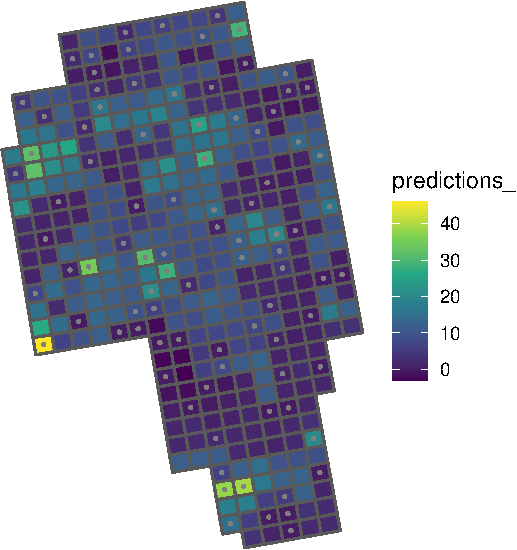
\includegraphics{preprint_springer_files/figure-latex/unnamed-chunk-8-1.pdf}
\caption{\label{fig:sitepredmap} A map of the sites composing the Taylor
corridor in eastern-central Alaska. Each site is roughly 4 kilometers in
length and roughly 3.5 kilometers in width so that the centroids of two
horizontally adjacent sites are about 4 kilometers apart and the
centroids of two vertically adjacent sites are about 3.5 kilometers
apart. (a). A map of the stratification for the sites in the year 2020.
(b). A map of the predictions of sites in 2020 from the spatio-temporal
model. A site with a grey dot in the center means that the site was
sampled in 2020.}
\end{figure}

In each year of the survey, a team of biologists stratifies all of the
spatial sites into a ``High'' stratum and a ``Low'' stratum based on
wildlife biologist knowledge of moose density in the region and counts
from previous surveys, which sites have land cover more suitable to
moose habitat, and, in some years, stratification flights done on a
portion of the region of interest prior to that year's survey (Figure
\ref{fig:sitepredmap}). The stratification scheme therefore can change
from year to year, though the majority of spatial sites are classified
into the same stratum in every year. Biologists then randomly select
some of the 381 sites to survey, and subsequently select a few
additional sites non-randomly in such a way that there are no large
areas in the region of interest without a sampled site. The non-randomly
selected sites are a small proportion of the overall sample size (about
10-15\% of the sites are selected non-randomly), and these sites are not
selected preferentially by the number of expected moose or observed
moose counts in previous survey years. The operations manual by Kellie
and DeLong (2006) provides more details about how sites are selected for
a survey in a particular year. The total number of sites that were
selected varies from a low of 76 in the year 2019 to a high of 90 in the
year 2020. Throughout the 7 unique years, some sites were sampled as
many as five different times while others were never sampled at all. The
number of units sampled throughout all survey years, \(n\), was 487
units. Figure \ref{fig:sitepredmap} and all remaining figure graphics
are constructed with the \(\texttt{ggplot2 R}\) package (Wickham 2016).

The goal of the following analysis is to predict the total abundance of
moose across all sites in the year 2020, the most recent year of the
survey, using stratum as a covariate in the spatio-temporal model.

\hypertarget{subsection:modelfit}{%
\subsection{Model Fitting}\label{subsection:modelfit}}

We fit the product-sum covariance model defined in equation
\ref{equation:model} using REML with stratum as a covariate in the
design matrix. To select the spatial and temporal correlation
structures, we examined the AIC values for each of the nine crossed
combinations of the exponential, spherical, and gaussian spatial
correlation structures (Cressie 2015) and the exponential, spherical,
and gaussian temporal correlation structures to assess model fit. The
combination with the lowest AIC was the ``gaussian spatial - exponential
temporal'' model. However, in this application, we opt to use the
``exponential spatial - exponential temporal'' model, with the
exponential spatial correlation structure defined in equation
\ref{equation:spatcov} and the exponential temporal correlation
structure defined in equation \ref{equation:tempcov} so that the
application correlation structure matches that of the simulations in
Section \ref{section:Simulation} (which are easier to conceptualize when
both the spatial and temporal correlations decay according to the same
function). Additionally, the AIC value for this ``exponential spatial -
exponential temporal'' model was within four points of the best model,
indicating that the quality of the model fits are not too different
anyway.

Table \ref{tab:paramest} gives the estimated parameters from the model
fit with the exponential correlation structures.

\begin{table}[H]

\caption{\label{tab:paramest}Estimated covariance parameters in the model. $\hat{\sigma}^2_{\delta}$, $\hat{\sigma}^2_{\gamma}$, and $\hat{\phi}$ are the spatial dependent error variance, independent error variance, and range parameters, respectively. $\hat{\sigma}^2_{\tau}$, $\hat{\sigma}^2_{\eta}$, and $\hat{\rho}$ are the temporal dependent error variance, independent error variance, and range parameters, respectively. $\hat{\sigma}^2_{\omega}$ and $\hat{\sigma}^2_{\nu}$ are the spatio-temporal dependent error variance and spatio-temporal independent error variance.}
\centering
\begin{tabular}[t]{cccccccc}
\toprule
\multicolumn{3}{c}{Spatial} & \multicolumn{3}{c}{Temporal} & \multicolumn{2}{c}{Spatio-temporal} \\
\cmidrule(l{3pt}r{3pt}){1-3} \cmidrule(l{3pt}r{3pt}){4-6} \cmidrule(l{3pt}r{3pt}){7-8}
$\hat{\sigma}^2_{\delta}$ & $\hat{\sigma}^2_{\gamma}$ & $\hat{\phi}$ & $\hat{\sigma}^2_{\tau}$ & $\hat{\sigma}^2_{\eta}$ & $\hat{\rho}$ & $\hat{\sigma}^2_{\omega}$ & $\hat{\sigma}^2_{\nu}$\\
\midrule
16.37 & 7.78 & 4.51 & 0.29 & 0 & 3.68 & 25.53 & 36.47\\
\bottomrule
\end{tabular}
\end{table}

To help interpret what some of these fitted covariance parameter
estimates mean, we can construct a fitted covariance plot (Figure
\ref{fig:covplot}). As the spatial distance between the centroids of two
sites increases (dark colour to light colour), the covariance of two
random errors decreases to 0, with the \(\hat{\phi}\) parameter estimate
controlling the rate of decay. In fact, the model estimates the
covariance to be nearly 0 when the centroids of two sites are 20 or more
kilometers apart, no matter what the temporal distance is. The
covariance between two errors that are six years apart is still
estimated to be positive if the two errors come from the same site or
from adjacent sites.

\begin{figure}
\centering
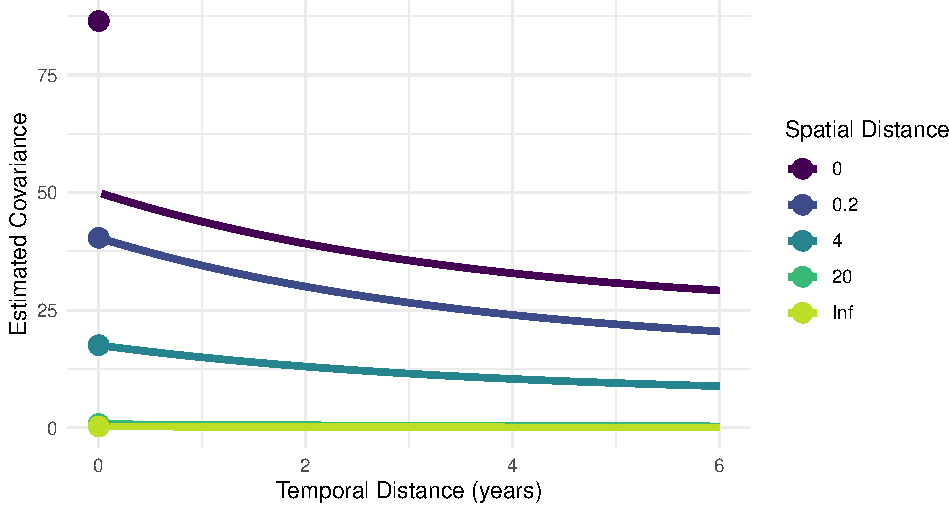
\includegraphics{preprint_springer_files/figure-latex/covplot-1.pdf}
\caption{\label{fig:covplot} Estimated covariance of the errors from the
estimated parameters in a spatio-temporal product-sum model. Distance
between two sites is calculated from the site centroids; the centroids
of two sites directly adjacent to one another are about 3.5 to 4
kilometers apart.}
\end{figure}

The estimated vector of fixed effects, using ``High'' as the reference
group, is \(\bm{\hat{\beta}}'\) = \((\hat{\beta}_0, \hat{\beta}_1)\) =
(9.62, -4.55). The standard error for \(\hat{\beta}_0\) is 1.01 while
the standard error for \(\hat{\beta}_1\) is 0.93. Therefore, the overall
mean for sites in the ``High'' stratum is estimated to be 9.62 moose
while the overall mean for sites in the ``Low'' stratum is estimated to
be 5.07 moose.

\hypertarget{prediction}{%
\subsection{Prediction}\label{prediction}}

We now use the fitted spatio-temporal model with the BLUP from equation
\ref{equation:blup} and weights given in equation
\ref{equation:currentweights} to predict the total abundance across all
sites in the year 2020, the most recent year of the survey. Plugging in
estimates of the covariance parameters into equations
\ref{equation:blup} and \ref{equation:predvar} and letting elements of
\(\mathbf{b}_a\) be equal to 1 for data points in 2020 and equal to 0
otherwise, we obtain a prediction of 3001 moose and a standard error
(the square root of the prediction variance) of 217 moose. The
prediction for the total and the prediction variance were fairly robust
to other combinations of correlation functions to model the spatial and
the temporal correlation, with the prediction never deviating from 3001
by more than 100 moose for any of the other 8 spatial and temporal
correlation function combinations discussed at the beginning of
Subsection \ref{subsection:modelfit}.

A 90\% normal-based prediction interval for the total abundance in 2020
(with the exponential spatial and temporal correlation) is (2644, 3357)
moose. Note that, though the response in this example is a count, a
normal-based prediction interval for the total is still appropriate
through an application of the central limit theorem for dependent data
(Smith 1980). Sitewise predictions for sites in 2020 are given in the
map in Figure \ref{fig:sitepredmap}.

For comparison, we use the spatial \texttt{sptotal} package (Higham, Ver
Hoef, Frank, et al. 2021) to compute the spatial FPBK prediction (Ver
Hoef 2008) for the total abundance of moose in the year 2020 with
stratum as a covariate. Note that the widely used GSPE software for
moose surveys allows for the strata to have different covariance
parameters and does not treat stratum as a covariate (DeLong 2006). For
the application of moose abundance prediction, analyzing each stratum
individually often results in better precision. The separate-stratum
analysis is discussed in more detail in the Supplementary Material in
the \protect\hyperlink{appendix}{Appendix}.

We also use the stratified random sampling design-based estimator
\mbox{} \begin{equation*}
\sum_{i = 1}^{2} N_i \cdot \bar{y}_i
\end{equation*} \noindent where \(\bar{y}_i\) is the sample mean for the
observed data in 2020 in the \(i^{th}\) stratum and \(N_i\) is the total
number of sites in 2020 in the \(i^{th}\) stratum. The stratified random
sampling design-based estimator has a variance for the total abundance
of \mbox{} \begin{equation*}
\sum_{i = 1}^{2} N_i^2 \cdot \left(1 - \frac{n_i}{N_i}\right) \cdot \frac{s^2_i}{n_i},
\end{equation*} \noindent where \(s^2_i\) is the sample variance of the
observed data points in 2020 in the \(i^{th}\) stratum and \(n_i\) is
the number of observed data points in 2020 in the \(i^{th}\) stratum.
Both the purely spatial model fit with \texttt{sptotal} and the
stratified random sampling design-based estimator use data only from
2020. Note that the stratified random sampling estimator is not actually
appropriate for this application because not all sites are randomly
selected within each stratum. However, the number of sites that are not
randomly selected is small, so we still include the stratified random
sampling estimator for a baseline comparison estimator.

For the purely spatial model with stratum as a covariate, the prediction
for the total number of moose in 2020 in the region is 2870 moose with a
standard error of 319 moose. For the stratified random sampling
design-based estimator, the estimated total number of moose in 2020 in
the region is 2853 moose with a standard error of 371 moose. While the
predictions for the total moose abundance are similar across the three
methods, we see that the spatio-temporal model is most efficient (\(SE\)
= 217 moose compared to 319 moose for the purely spatial model that
ignores previous surveys and 371 moose for the stratified random
sampling design-based estimator that ignores both previous surveys and
spatial correlation in the current survey).

In addition to making a prediction for the abundance in the most recent
survey, we can also use the spatio-temporal model to backcast
predictions for the abundance in past survey years, interpolate
predictions for years during which a survey was not completed, and
forecast predictions for future years. For example, in the Taylor
Corridor surveys, there was no survey conducted in the year 2016 because
of insufficient snow cover. Leveraging the temporal structure of the
ST-FPBK predictor, we can still construct a prediction and corresponding
standard error though, as expected, this standard error is larger than
the standard errors of years where a survey was completed (Figure
\ref{fig:trend}). Also, in Figure \ref{fig:trend}, we see a forecasted
prediction and corresponding standard error for the abundance in 2021.
Again, the standard error associated with the forecasted prediction is
larger than the standard errors for the years with completed surveys.

\begin{figure}
\centering
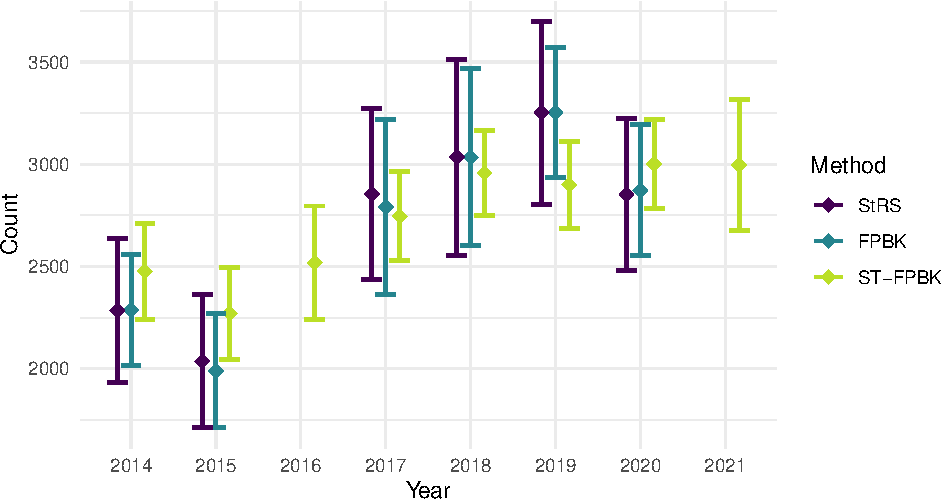
\includegraphics{preprint_springer_files/figure-latex/unnamed-chunk-13-1.pdf}
\caption{\label{fig:trend} Moose abundance predictions for the Taylor
Corridor from 2014 through 2021 with the stratified random sampling
(StRS) estimator, the spatial FPBK predictor, and the ST-FPBK predictor.
Predictions are given with a diamond symbol; the bars surrounding each
prediction are standard error bars. Because surveys were not conducted
in 2016 and 2021, there is no StRS estimator or spatial FPBK predictor
for those years. Also, the standard errors for the ST-FPBK predictor for
those years is larger than the standard errors in the other years. The
stratification scheme used for 2016 and 2021 in the ST-FPBK analysis was
the same scheme used in 2015 and 2020, respectively.}
\end{figure}

\hypertarget{section:Simulation}{%
\section{Simulation}\label{section:Simulation}}

\hypertarget{description}{%
\subsection{Description}\label{description}}

To evaluate performance of the ST-FPBK predictor, we conduct a
simulation study. We simulate a response vector \(\mathbf{y}\) of length
\(N = 1000\) on a \(10 \times 10\) grid of 100 spatial sites on the unit
square (\([0, 1] \times [0, 1]\)) and 10 equally-spaced time points in
the interval \([0, 1]\), so that each spatial site has a response value
at each time point. The random vector \(\mathbf{y}\) is multivariate
normal with mean \(\mathbf{0}\) and product-sum covariance matrix
\(\bm{\Sigma}\) defined in equation \ref{equation:var} with the
covariance parameters given in Table \ref{tab:simparmtab}.

\begin{table}[H]

\caption{\label{tab:simparmtab}Covariance parameters used to simulate data. $\sigma^2_{\delta}$, $\sigma^2_{\gamma}$, and $\phi$ are the spatial dependent error variance, independent error variance, and range parameters, respectively. $\sigma^2_{\tau}$, $\sigma^2_{\eta}$, and $\rho$ are the temporal dependent error variance, independent error variance, and range parameters, respectively. $\sigma^2_{\omega}$ and $\sigma^2_{\nu}$ are the spatio-temporal dependent error variance and spatio-temporal independent error variance. Note that both $\phi$ (and $\rho$) appear in $\mathbf{R}_{st}$; therefore, their values can change the underlying covariance even when $\sigma^2_{\delta}$ (and $\sigma^2_{\tau}$) are equal to 0.}
\centering
\begin{tabular}[t]{ccccccccc}
\toprule
\multicolumn{1}{c}{ } & \multicolumn{3}{c}{Spatial} & \multicolumn{3}{c}{Temporal} & \multicolumn{2}{c}{Spatio-temporal} \\
\cmidrule(l{3pt}r{3pt}){2-4} \cmidrule(l{3pt}r{3pt}){5-7} \cmidrule(l{3pt}r{3pt}){8-9}
scenario & $\sigma^2_{\delta}$ & $\sigma^2_{\gamma}$ & $\phi$ & $\sigma^2_{\tau}$ & $\sigma^2_{\eta}$ & $\rho$ & $\sigma^2_{\omega}$ & $\sigma^2_{\nu}$\\
\midrule
all-dev & 0.5 & 0.17 & 0.47 & 0.5 & 0.17 & 0.33 & 0.50 & 0.17\\
t-iev & 0.0 & 0.00 & 0.47 & 0.0 & 1.50 & 0.00 & 0.25 & 0.25\\
spt-iev & 0.0 & 0.00 & 0.00 & 0.0 & 0.00 & 0.00 & 0.00 & 2.00\\
\bottomrule
\end{tabular}
\end{table}

The three scenarios in Table \ref{tab:simparmtab} correspond to (1)
\textbf{all-dev}: a scenario where a substantial proportion of the
overall variance comes from the spatial, temporal, and spatio-temporal
dependent error variance parameters
\(\sigma^2_{\delta}, \sigma^2_{\tau},\) and \(\sigma^2_{\omega}\); (2)
\textbf{t-iev}: a scenario where there the overall variance is dominated
by the temporal independent error variance parameter,
\(\sigma^2_{\eta}\); and (3) \textbf{spt-iev}: a scenario where all of
the variability comes from \(\sigma^2_{\nu}\) so that errors are
independent regardless of spatial and time indices. In all scenarios,
summing all six variance parameters gives a total variance equal to two.

Both \(\mathbf{R}_{s}\) and \(\mathbf{R}_t\) are generated from the
exponential correlation function with \(\phi\) and \(\rho\) as the range
parameters in equations \ref{equation:spatcov} and
\ref{equation:tempcov}. The values \(0.471\) and \(0.3333\) are chosen
for \(\phi\) and \(\rho\), respectively, so that the effective ranges,
\(3 \phi\) and \(3 \rho\), are equal to the maximum distance between two
data points in space (\(\sqrt2 = 1.414\)) and the maximum distance
between two data points in time (\(1\)). A value of 0 for \(\phi\) (or
\(\rho\)) sets the \(\mathbf{R}_{s}\) (or the \(\mathbf{R}_t\)) matrix
to the identity matrix. Figure \ref{fig:simcovplot} shows the model
covariance of the errors used to generate data for the ``all-dev''
scenario.

\begin{figure}
\centering
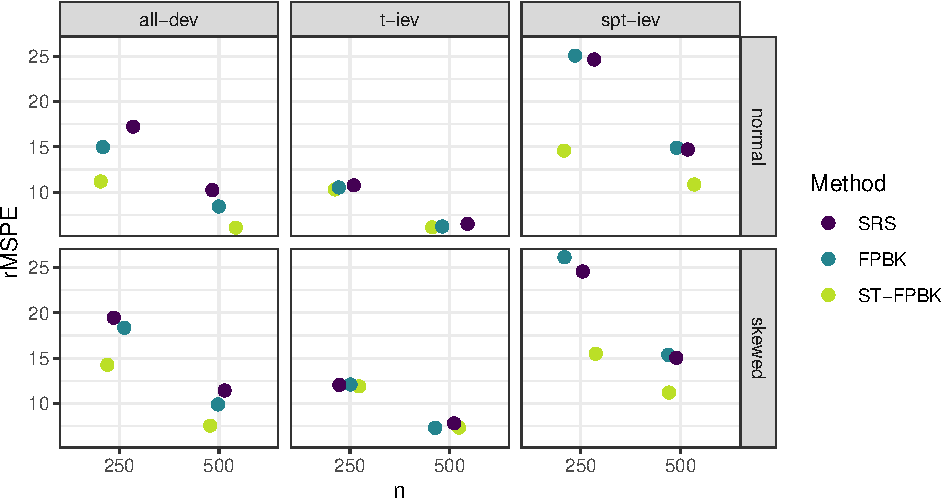
\includegraphics{preprint_springer_files/figure-latex/unnamed-chunk-17-1.pdf}
\caption{\label{fig:simcovplot} The model covariance used in the
simulations for the spatio-temporal scenario. Covariance is
approximately 0 for errors from data points that are \(\sqrt2\) distance
units apart in space and 1 distance unit apart in time. The spatial
dependent error variance (\(\sigma^2_{\delta}\)), spatial independent
error variance (\(\sigma^2_{\gamma}\)), temporal dependent error
variance (\(\sigma^2_{\tau}\)), and temporal independent error variance
(\(\sigma^2_{\eta}\)) are shown with grey lines.}
\end{figure}

Each of these three scenarios is replicated for two different sample
sizes: \(n = 250\) and \(n = 500\). A simple random sample is chosen
from the 1000 total data points.

Finally, the simulation experiment is repeated for a continuous skewed
response variable and for a skewed response variable of discrete counts.
To create the continuous skewed response variable for the setting called
``skewed,'' a normally-distributed response is simulated according to
the parameters given in Table \ref{tab:simparmtab}, except that each of
the variance parameters (not including \(\phi\) and \(\rho\)) is divided
by 2.89 so that the total variance is equal to 0.6931. This variable is
then exponentiated so that the total variance after exponentiation is
equal to 2. Note that, not only does exponentiation result in a
right-skewed response variable, but exponentiating also allows for an
assessment of how the ST-FPBK predictor performs when the covariance is
mis-specified, as the resulting response variable is now simulated with
an intractable covariance function that is not used in the model
fitting. To create the skewed response variable of discrete counts for
the setting called ``poisson,'' for each response value, we take a
Poisson draw with the continuous skewed response value as the mean
(conditional on the mean, each Poisson draw is done independently of all
other Poisson draws).

Therefore, the simulation study has \(18\) total settings coming from a
\(3 \times 2 \times 3\) (scenario \(\times\) sample size \(\times\)
distribution) factorial design. For each setting, we simulate 1000
realizations of the response vector \(\mathbf{y}\). For each
realization, we use three methods to predict the total response for the
``most current'' time point, which is when the time index is equal to 1
on the interval \([0, 1]\)). We will henceforth call this ``total
response for the most current time point quantity'' the ``current
total.''

The first method uses the ST-FPBK predictor in equation
\ref{equation:blup} with the spatio-temporal model covariance in
equation \ref{equation:var}. REML estimation with the observed data
\(\mathbf{y}_o\) is used to obtain estimates for the covariance
parameter vector \(\bm{\theta}\). The second method is the FPBK spatial
model fit with the \texttt{sptotal R} package (Higham, Ver Hoef, Frank,
et al. 2021) that only uses data from the most current time point.

The third method uses a simple random sample (SRS) design-based
estimator with data from the most current time point. The SRS
design-based estimator for the total is \(100 \cdot \bar{y}\), where
\(\bar{y}\) is the sample mean of the response in the most current time
point. The variance of the estimator (Lohr 2021) is
\(100^2 \cdot \frac{s^2}{n_1} \cdot (1 - \frac{n_1}{100})\), where
\(s^2\) is the sample variance of the response variable in the most
current time point and \(n_1\) is the number of sampled locations in the
most current time point.

The SRS method gives an estimator, not a predictor, and a corresponding
confidence interval, not a prediction interval, because the SRS
design-based estimator treats the observed data as fixed, not as a
random realization from a process (Brus 2021; Dumelle et al. 2022).
However, in the remaining text and tables, we refer to the ``current
total'' response quantity obtained from the three methods as a
``prediction'' and to the corresponding interval as a ``prediction
interval'' to limit unnecessarily verbose text and tables.

For each method, we calculate the root-mean-squared-prediction-error
(rMSPE) as
\(\sqrt{\frac{1}{1000}(\sum_{i = 1}^{1000}(T_i - \hat{T}_i)^2)}\), where
\(T_i\) and \(\hat{T}_i\) are the realized and predicted current totals,
respectively, in the \(i^{th}\) iteration. Bias is recorded as
\(\frac{1}{1000}\sum_{i = 1}^{1000}(T_i - \hat{T}_i)\). We also create a
normal-based 90\% prediction interval for the realized current total and
record \(\frac{1}{1000} \sum_{i = 1}^{1000}I(LB_i < T_i < UB_i)\), where
\(I(LB_i < T_i < UB_i)\) is an indicator variable that is equal to \(1\)
if the realized total in iteration \(i\), \(T_i\), is between the lower
bound, \(LB_i\), and the upper bound, \(UB_i\), of the \(i^{th}\)
prediction interval.

\hypertarget{results}{%
\subsection{Results}\label{results}}

Tables \ref{tab:simrmspetab}, \ref{tab:simbiastab}, and
\ref{tab:simpitab} in the \protect\hyperlink{appendix}{Appendix} give
the rMSPE, bias, and interval coverage of the three methods in all 18
simulation settings. In Figure \ref{fig:rmspe}, we see that the ST-FPBK
predictor outperforms both the purely spatial FPBK predictor and the
simple random sample design-based estimator in all of the ``all-dev''
and ``spt-iev'' scenarios. In general, rMSPE improvement is larger for
the smaller sample size.

We see little gains in rMSPE for the ST-FPBK predictor in the ``t-iev''
scenario. This setting was chosen to explore how the spatio-temporal
model would perform when most of the variability in the response comes
from \(\sigma^2_{\eta}\). In this scenario, the mean of the response,
conditional on the random effects, can fluctuate drastically from time
point to time point. Therefore, in a model without any fixed effects,
the realized total is susceptible to time point to time point increases
and decreases more than the realized total is in the other scenarios. As
expected, the ST-FPBK predictor performs no better than a purely spatial
model or the SRS design-based estimator for the ``t-iev'' scenario
because the information from data in other time points is not as useful.
However, we can also say that the added complexity of the
spatio-temporal model is not detrimental.

\begin{figure}
\centering
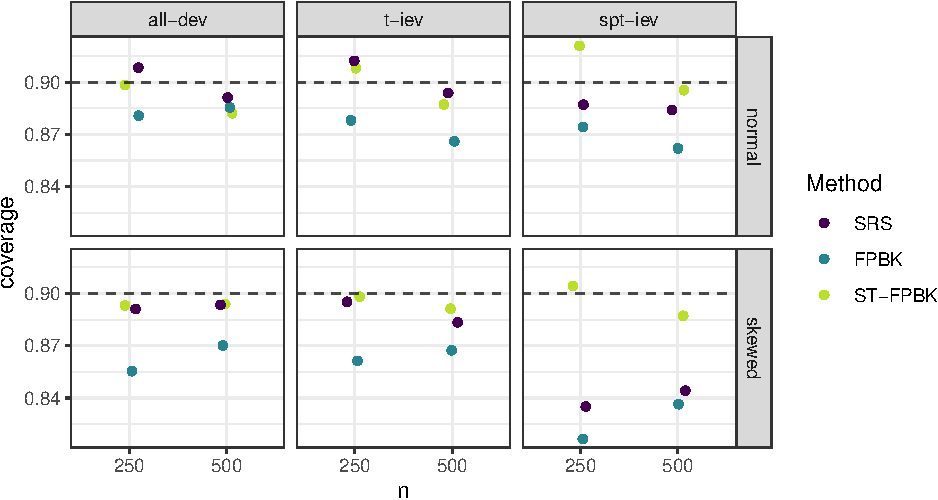
\includegraphics{preprint_springer_files/figure-latex/unnamed-chunk-19-1.pdf}
\caption{\label{fig:rmspe} root-mean-squared-prediction-error (rMSPE)
for all simulation settings. The ST-FPBK predictor has the smallest
rMSPE in all of the `all-dev' and `spt-iev' scenarios while the three
methods perform similarly in all of the `t-iev' scenarios.}
\end{figure}

All methods appear relatively unbiased in all simulation settings: Table
\ref{tab:simbiastab} shows that the bias of each method is small
compared to the squares of the rMSPE values given in Table
\ref{tab:simrmspetab}.

The normal-based prediction intervals (Smith 1980) for the abundance in
the most recent time point from the ST-FPBK method maintain close to
appropriate coverage (90\%) for all of the simulation settings used,
including the scenarios where the response is skewed right and the
covariance model is mis-specified and the scenarios where the response
is both discrete and skewed right (Table \ref{tab:simpitab}). The
spatial model and the SRS design-based estimator have lower than nominal
coverage in some settings because of the small sample size used (recall
that the \(n = 250\) observed samples span 10 unique time points so
that, on average, the spatial model and SRS design-based estimator only
have 25 observed responses to use in the current time point).

\hypertarget{section:Discussion}{%
\section{Discussion}\label{section:Discussion}}

We see in the moose application in Section \ref{section:Application}
that there is substantial reduction in the standard error of the
predictor for the total moose abundance in 2020 when incorporating data
from surveys in previous years. In the simulation study in Section
\ref{section:Simulation}, we find that the ST-FPBK predictor has lower
rMSPE than the FPBK predictor from a purely spatial model and an SRS
design-based estimator in many settings. The ST-FPBK predictor is less
beneficial when the temporal independent error variance contributes a
large proportion to the overall variance. Additionally, the ST-FPBK
predictor maintains appropriate interval coverage in all settings
tested, even when the covariance for the errors is mis-specified or the
response is discrete.

An additional possible benefit of using the ST-FPBK predictor compared
to a purely spatial FPBK predictor is the potential for forecasting
abundance before a survey is completed. In Figure \ref{fig:trend}, we
see the forecasted prediction for abundance in the year 2021. While
there is a (presumed) loss in precision by constructing a prediction for
a year that has no observed samples, the prediction could still be
useful to wildlife managers for decision-making before a survey from
that year is completed and analyzed. Constructing a prediction for years
or time points at which a survey is not completed can be applied to
other contexts as well, including temporal interpolation (e.g., the year
2016 in Figure \ref{fig:trend}).

The ability to predict the abundance (or other quantity) in time points
that were not surveyed also allows biologists to investigate how much
efficiency is lost from, for example, sampling every other year instead
of every year. These types of surveys are often expensive, so perhaps
the drop in efficiency from sampling every other year is worth the cost
of completing those surveys annually.

We would also like to give our perception of the benefits and drawbacks
of our approach with using a Bayesian hierarchical model. For example,
Schmidt et al. (2022) use a Bayesian hierarchical model with spatial
radial basis functions that are estimated per year and with time as a
trend component in the fixed effects to make predictions for moose
abundance. We argue that our approach is both simpler for practitioners
and less likely to yield an unreasonable abundance prediction, compared
to a Bayesian hierarchical model. In general, fitting a Bayesian
hierarchical model with a complex covariance structure on the link scale
requires careful thought in formulating the model and the prior
distributions used for all of the covariance parameters used to model
covariance on the link scale (Conn et al. 2015).

Conn et al. (2015) also note that the need to tailor the model used to
the richness of the particular data set at hand is especially important
when using the log link function, as abundance estimates can become
unrealistically large when back-transforming. Indeed, Ver Hoef et al.
(2021) fit a Bayesian hierarchical model to marine mammal counts using a
truncated normal distribution for the random errors on the log scale
instead of the typical normal distribution. Applying a Bayesian
hierarchical model to this data set with normally distributed random
errors on the link scale and non-informative prior distributions
resulted in predicted counts well above what any biologist familiar with
the region would consider reasonable. Conn et al. (2014) and Ver Hoef
and Jansen (2007) provide more evidence that applying a hierarchical
model with a log link function could result in unrealistically high
predictions, particularly when a small proportion of the region of
interest is sampled. All of these examples indicate that a Bayesian
hierarchical model may need significant adjustment based on the
particular data set at hand.

Another benefit of our approach is a faster fitting time, as there is no
need to construct and implement the time-consuming Markov chain Monte
Carlo sampler. The moose application model in Section
\ref{section:Application} takes about 10 minutes to fit. There is a
trade-off here between how many surveys to incorporate into the model
(the Alaska Department of Fish and Game has done surveys with this
structure since the late 1990's) and how long the model will take to
fit. We expect there to be diminishing returns in precision when
incorporating older surveys, though the rate at which the returns
diminish is dependent upon the application at hand. Additionally, with
the shorter fitting time and the supplementary \texttt{R} package
provided to fit the models, integrating this approach with the current
GSPE software would be more reasonable and would also allow scientists
other than statisticians to perform the analysis. Finally, our approach
is easier to assess in a simulation study, which would be too
time-prohibitive for the Bayesian model. Biometricians could use
simulation with our approach to answer various questions given proposed
values of covariance parameters like how much efficiency would drop if a
survey was only conducted every other year.

Bayesian hierarchical models, including the model by Schmidt et al.
(2022), however, offer features that would be harder to implement in our
approach. These models allow for incorporation of more levels in the
model structure, allowing, for example, for imperfect detection of
animals from a separate detectability survey. Additionally, the Bayesian
hierarchical model can use a Poisson or negative binomial model for the
counts. Therefore, an appropriate prediction interval for the response
on one particular site could be constructed. On the other hand, for our
approach, we rely on the central limit theorem for dependent data to
form a prediction interval for the total, which would not apply to a
prediction interval for the response on just one site.

We have developed a finite population block kriging predictor for
spatio-temporal data, which adjusts the variance of the predictor to be
appropriate for sampling from a finite population. The resulting
predictor is generally at least as good as the predictor from a purely
spatial model, and, is often much better. Monitoring programs that use
regularly scheduled surveys should consider incorporating data from past
surveys to improve precision in the predictor for the most current
survey.

Future work in this area includes developing a frequentist model for
which imperfect detection of units through time is incorporated into the
predictor (Higham, Ver Hoef, Madsen, et al. 2021) or how best to select
sites to sample for future surveys given proposed values for the
spatio-temporal covariance parameters. Additionally, for moose surveys
in particular, updating the GSPE software to include analysis for
spatio-temporal data could be useful for practitioners. Though we
recognize that doing so would be a substantial undertaking, the
\texttt{R} package that we provide could be a useful starting point for
the integration.

\hypertarget{declarations}{%
\section{Declarations}\label{declarations}}

\hypertarget{conflicts-of-interest}{%
\subsection*{Conflicts of Interest}\label{conflicts-of-interest}}
\addcontentsline{toc}{subsection}{Conflicts of Interest}

The authors declare no conflict of interest.

\hypertarget{data-and-code-availability}{%
\subsection*{Data and Code
Availability}\label{data-and-code-availability}}
\addcontentsline{toc}{subsection}{Data and Code Availability}

The Alaska Department of Fish and Game collected and provided the moose
survey data used in this study. This manuscript has a supplementary
\texttt{R} package that contains all of the data and code used in its
creation, with the exception of the shapefile used to make the maps in
some of the figures (which cannot be released due to Alaska Department
of Fish and Game policy). The supplementary \texttt{R} package, along
with the data used in the application, is hosted on GitHub and can be
found at (link not provided because repository would identify at least
one author).

The data set is also available on Zenodo at
\url{https://doi.org/10.5281/zenodo.7636130}.

\hypertarget{acknowledgements}{%
\subsection*{Acknowledgements}\label{acknowledgements}}
\addcontentsline{toc}{subsection}{Acknowledgements}

The views expressed in this manuscript are those of the authors and do
not necessarily represent the views or policies of the U.S.
Environmental Protection Agency or the National Oceanic and Atmospheric
Administration. Any mention of trade names, products, or services does
not imply an endorsement by the U.S. government, the U.S. Environmental
Protection Agency, or the National Oceanic and Atmospheric
Administration. The U.S. Environmental Protection Agency and National
Oceanic and Atmospheric Administration do not endorse any commercial
products, services, or enterprises.

\setcounter{table}{0}
\setcounter{subsection}{0}
\renewcommand{\thetable}{A\arabic{table}}
\renewcommand{\thesubsection}{A.\arabic{subsection}:}

\hypertarget{appendix}{%
\section*{Appendix}\label{appendix}}
\addcontentsline{toc}{section}{Appendix}

\subsection{Simulation Tables}

\begin{table}[H]

\caption{\label{tab:simrmspetab}root-mean-squared-prediction-error (rMSPE) for the ST-FPBK predictor, the FPBK predictor, and the SRS estimator for each of the 18 simulation settings. In all settings, the rMSPE for the ST-FPBK predictor is approximately equal to or lower than the rMSPE for the other two methods.}
\centering
\begin{tabular}[t]{cccccc}
\toprule
\multicolumn{3}{c}{Simulation Setting} & \multicolumn{3}{c}{rMSPE} \\
\cmidrule(l{3pt}r{3pt}){1-3} \cmidrule(l{3pt}r{3pt}){4-6}
scenario & n & Response Type & SRS & FPBK & ST-FPBK\\
\midrule
spt-iev & 250 & normal & 24.85 & 25.19 & 14.99\\
t-iev & 250 & normal & 11.44 & 11.01 & 10.88\\
all-dev & 250 & normal & 17.91 & 15.33 & 11.38\\
\midrule
spt-iev & 500 & normal & 14.53 & 14.63 & 11.06\\
t-iev & 500 & normal & 6.55 & 6.10 & 6.05\\
all-dev & 500 & normal & 9.68 & 8.13 & 5.87\\
\midrule
spt-iev & 250 & skewed & 26.21 & 27.28 & 15.73\\
t-iev & 250 & skewed & 12.60 & 12.98 & 12.69\\
all-dev & 250 & skewed & 21.42 & 19.10 & 16.19\\
\midrule
spt-iev & 500 & skewed & 14.86 & 15.01 & 10.91\\
t-iev & 500 & skewed & 7.45 & 6.84 & 6.80\\
all-dev & 500 & skewed & 11.75 & 10.71 & 8.68\\
\midrule
spt-iev & 250 & poisson & 33.63 & 34.57 & 20.19\\
t-iev & 250 & poisson & 24.39 & 25.84 & 24.73\\
all-dev & 250 & poisson & 30.78 & 29.32 & 27.14\\
\midrule
spt-iev & 500 & poisson & 18.60 & 18.84 & 14.21\\
t-iev & 500 & poisson & 14.13 & 14.09 & 13.82\\
all-dev & 500 & poisson & 17.12 & 16.99 & 15.90\\
\bottomrule
\end{tabular}
\end{table}

\begin{table}[H]

\caption{\label{tab:simbiastab}Bias (Realized Current Total - Predicted Current Total) for the ST-FPBK predictor, the FPBK predictor, and the SRS estimator for each of the 18 simulation settings. In all settings, all methods appear fairly unbiased.}
\centering
\begin{tabular}[t]{cccccc}
\toprule
\multicolumn{3}{c}{Simulation Setting} & \multicolumn{3}{c}{Bias} \\
\cmidrule(l{3pt}r{3pt}){1-3} \cmidrule(l{3pt}r{3pt}){4-6}
scenario & n & Response Type & SRS & FPBK & ST-FPBK\\
\midrule
spt-iev & 250 & normal & -0.40 & -0.63 & 0.34\\
t-iev & 250 & normal & -0.28 & -0.48 & -0.38\\
all-dev & 250 & normal & -0.30 & -0.45 & -0.36\\
\midrule
spt-iev & 500 & normal & -0.30 & -0.35 & 0.05\\
t-iev & 500 & normal & -0.20 & -0.21 & -0.20\\
all-dev & 500 & normal & 0.11 & -0.08 & -0.19\\
\midrule
spt-iev & 250 & skewed & -0.58 & -1.72 & -0.14\\
t-iev & 250 & skewed & -0.49 & -1.02 & -0.82\\
all-dev & 250 & skewed & -0.19 & -0.74 & -0.47\\
\midrule
spt-iev & 500 & skewed & -0.44 & -0.69 & -0.15\\
t-iev & 500 & skewed & -0.23 & -0.33 & -0.30\\
all-dev & 500 & skewed & 0.18 & -0.08 & -0.01\\
\midrule
spt-iev & 250 & poisson & -0.72 & -1.79 & -0.03\\
t-iev & 250 & poisson & -0.70 & -1.25 & -1.01\\
all-dev & 250 & poisson & -0.52 & -1.34 & -0.67\\
\midrule
spt-iev & 500 & poisson & -0.28 & -0.43 & 0.07\\
t-iev & 500 & poisson & -0.61 & -0.69 & -0.61\\
all-dev & 500 & poisson & 0.57 & 0.30 & 0.61\\
\bottomrule
\end{tabular}
\end{table}

\begin{table}[H]

\caption{\label{tab:simpitab}Prediction interval coverage for the ST-FPBK predictor, the FPBK predictor, and the SRS for each of the 18 simulation settings. All intervals are normal-based and have a nominal coverage level of 0.90.}
\centering
\begin{tabular}[t]{cccccc}
\toprule
\multicolumn{3}{c}{Simulation Setting} & \multicolumn{3}{c}{Coverage} \\
\cmidrule(l{3pt}r{3pt}){1-3} \cmidrule(l{3pt}r{3pt}){4-6}
scenario & n & Response Type & SRS & FPBK & ST-FPBK\\
\midrule
spt-iev & 250 & normal & 0.89 & 0.88 & 0.91\\
t-iev & 250 & normal & 0.88 & 0.87 & 0.89\\
all-dev & 250 & normal & 0.88 & 0.87 & 0.90\\
\midrule
spt-iev & 500 & normal & 0.89 & 0.88 & 0.90\\
t-iev & 500 & normal & 0.89 & 0.88 & 0.89\\
all-dev & 500 & normal & 0.91 & 0.88 & 0.90\\
\midrule
spt-iev & 250 & skewed & 0.86 & 0.83 & 0.90\\
t-iev & 250 & skewed & 0.88 & 0.86 & 0.90\\
all-dev & 250 & skewed & 0.86 & 0.86 & 0.89\\
\midrule
spt-iev & 500 & skewed & 0.86 & 0.86 & 0.90\\
t-iev & 500 & skewed & 0.89 & 0.88 & 0.92\\
all-dev & 500 & skewed & 0.89 & 0.86 & 0.90\\
\midrule
spt-iev & 250 & poisson & 0.86 & 0.84 & 0.91\\
t-iev & 250 & poisson & 0.89 & 0.87 & 0.90\\
all-dev & 250 & poisson & 0.87 & 0.86 & 0.85\\
\midrule
spt-iev & 500 & poisson & 0.88 & 0.87 & 0.90\\
t-iev & 500 & poisson & 0.89 & 0.88 & 0.91\\
all-dev & 500 & poisson & 0.87 & 0.86 & 0.88\\
\bottomrule
\end{tabular}
\end{table}

\subsection{Supplementary Analysis}

As mentioned in Section \ref{section:Application}, moose surveys in
Alaska are often stratified into ``High'' and ``Low'' sites. When using
stratum as a covariate in a spatio-temporal (or spatial, if performing a
purely spatial analysis) model, we assume that all errors in the model
are generated from the same underlying spatio-temporal (or spatial)
parameters. However, for many moose surveys, it is more reasonable to
allow the sites in the High stratum to have a different set of
spatio-temporal (or spatial) parameters than the sites in the Low
stratum.

If we allow the strata to have different covariance parameters, then, to
construct the ST-FPBK predictor, we simply fit the model once for each
stratum. If we assume that there is no cross-covariance (i.e.~errors
from sites in different strata are not correlated), then the BLUP for
\(\mathbf{b}'_a \mathbf{y}_a\) is

\begin{equation} \label{equation:blup_strat}
\widehat{\mathbf{b}'_a \mathbf{y}_a} = \bm{\lambda}_{o, l}' \mathbf{y}_{o, l} + \bm{\lambda}_{o, h}' \mathbf{y}_{o, h},
\end{equation}

\noindent where \(\bm{\lambda}_{o, l}\) and \(\bm{\lambda}_{o, h}'\) are
the kriging weights for the Low and High strata, respectively (equation
\ref{equation:blup}), and \(\mathbf{y}_{o, l}\) and
\(\mathbf{y}_{o, h}\) are the vectors of observed responses for the Low
and High strata, respectively.

Again assuming that there is no cross-covariance, the prediction
variance is simply the sum of the prediction variances of
\(\bm{\lambda}_{o, l}' \mathbf{y}_{o, l}\) and
\(\bm{\lambda}_{o, h}' \mathbf{y}_{o, h}\) using equation
\ref{equation:predvar}.

We can use the purely spatial model and FPBK as well as the
spatio-temporal model and ST-FPBK to predict the total moose abundance
in 2020, using separate covariance models for the strata in the moose
data set in Section \ref{section:Application}. Table
\ref{tab:sepstratres} shows the results.

\begin{table}[H]

\caption{\label{tab:sepstratres}Prediction and standard error for total abundance in 2020 using a model that allows errors in separate strata to be modeled with different covariance parameters. For reference, the prediction and standard error from the models with stratum as a covariate are also given.}
\centering
\begin{tabular}[t]{ccc}
\toprule
method & Prediction & SE\\
\midrule
FPBK Sep. Strat. & 2900 & 297\\
ST-FPBK Sep. Strat. & 2867 & 242\\
\midrule
FPBK & 2870 & 319\\
ST-FPBK & 3001 & 217\\
\bottomrule
\end{tabular}
\end{table}

The spatio-temporal predictors still have a smaller standard error than
their purely spatial model counterparts. Interestingly, the purely
spatial FPBK predictor has a slightly lower standard error when fitting
strata separately while the ST-FPBK predictor has a slightly lower
standard error when using stratum as a covariate. Whether it makes more
sense for stratum to be a covariate or for the strata to be fit
separately is application dependent.

For the moose application data, fitting separate covariance models to
each stratum is probably the better choice, as the errors for sites in
the high stratum have much more overall variability than the errors in
the low stratum. However, we chose to have the separate-strata model in
the supplementary materials for two reasons. First, the method can be
applied to any data set with spatio-temporal covariance and a finite
number of sites, and applications in other domains may not have
stratification at all. Second, the syntax in the development of the
ST-FPBK predictor is much cleaner when stratum is treated as a covariate
than when the strata are fit separately. Using the model with stratum as
a covariate allows for a better focus on the proposed method itself.

\hypertarget{references}{%
\section*{References}\label{references}}
\addcontentsline{toc}{section}{References}

\hypertarget{refs}{}
\begin{CSLReferences}{1}{0}
\leavevmode\vadjust pre{\hypertarget{ref-adde2020predicting}{}}%
Adde, Antoine, Marcel Darveau, Nicole Barker, and Steven Cumming. 2020.
{``Predicting Spatiotemporal Abundance of Breeding Waterfowl Across
Canada: A Bayesian Hierarchical Modelling Approach.''} \emph{Diversity
and Distributions} 26 (10): 1248--63.

\leavevmode\vadjust pre{\hypertarget{ref-boertje2009managing}{}}%
Boertje, Rodney D, Mark A Keech, Donald D Young, Kalin A Kellie, and C
Tom Seaton. 2009. {``Managing for Elevated Yield of Moose in Interior
Alaska.''} \emph{The Journal of Wildlife Management} 73 (3): 314--27.

\leavevmode\vadjust pre{\hypertarget{ref-breidt2017model}{}}%
Breidt, F Jay, and Jean D Opsomer. 2017. {``Model-Assisted Survey
Estimation with Modern Prediction Techniques.''}

\leavevmode\vadjust pre{\hypertarget{ref-breivik2021predicting}{}}%
Breivik, Olav Nikolai, Fredrik Aanes, Guldborg Søvik, Asgeir Aglen,
Sigbjørn Mehl, and Espen Johnsen. 2021. {``Predicting Abundance Indices
in Areas Without Coverage with a Latent Spatio-Temporal Gaussian
Model.''} \emph{ICES Journal of Marine Science} 78 (6): 2031--42.

\leavevmode\vadjust pre{\hypertarget{ref-brus2021statistical}{}}%
Brus, Dick J. 2021. {``Statistical Approaches for Spatial Sample Survey:
Persistent Misconceptions and New Developments.''} \emph{European
Journal of Soil Science} 72 (2): 686--703.

\leavevmode\vadjust pre{\hypertarget{ref-chen2021space}{}}%
Chen, Wanfang, Marc G Genton, and Ying Sun. 2021. {``Space-Time
Covariance Structures and Models.''} \emph{Annual Review of Statistics
and Its Application} 8: 191--215.

\leavevmode\vadjust pre{\hypertarget{ref-conn2015using}{}}%
Conn, Paul B, Devin S Johnson, Jay M Ver Hoef, Mevin B Hooten, Joshua M
London, and Peter L Boveng. 2015. {``Using Spatiotemporal Statistical
Models to Estimate Animal Abundance and Infer Ecological Dynamics from
Survey Counts.''} \emph{Ecological Monographs} 85 (2): 235--52.

\leavevmode\vadjust pre{\hypertarget{ref-conn2014estimating}{}}%
Conn, Paul B, Jay M Ver Hoef, Brett T McClintock, Erin E Moreland, Josh
M London, Michael F Cameron, Shawn P Dahle, and Peter L Boveng. 2014.
{``Estimating Multispecies Abundance Using Automated Detection Systems:
Ice-Associated Seals in the Bering Sea.''} \emph{Methods in Ecology and
Evolution} 5 (12): 1280--93.

\leavevmode\vadjust pre{\hypertarget{ref-cressie2015statistics}{}}%
Cressie, Noel. 2015. \emph{Statistics for Spatial Data - Revised
Edition}. John Wiley \& Sons.

\leavevmode\vadjust pre{\hypertarget{ref-cressie1993asymptotic}{}}%
Cressie, Noel, and Soumendra Nath Lahiri. 1993. {``The Asymptotic
Distribution of REML Estimators.''} \emph{Journal of Multivariate
Analysis} 45 (2): 217--33.

\leavevmode\vadjust pre{\hypertarget{ref-cressie2015statisticsspt}{}}%
Cressie, Noel, and Christopher K Wikle. 2015. \emph{Statistics for
Spatio-Temporal Data}. John Wiley \& Sons.

\leavevmode\vadjust pre{\hypertarget{ref-davy2021estimation}{}}%
Davy, Christina M, Kelly Squires, and J Ryan Zimmerling. 2021.
{``Estimation of Spatiotemporal Trends in Bat Abundance from Mortality
Data Collected at Wind Turbines.''} \emph{Conservation Biology} 35 (1):
227--38.

\leavevmode\vadjust pre{\hypertarget{ref-de2001product}{}}%
De Cesare, Luigi, DE Myers, and D Posa. 2001. {``Product-Sum Covariance
for Space-Time Modeling: An Environmental Application.''}
\emph{Environmetrics: The Official Journal of the International
Environmetrics Society} 12 (1): 11--23.

\leavevmode\vadjust pre{\hypertarget{ref-de2001space}{}}%
De Iaco, Sandra, Donald E Myers, and Donato Posa. 2001. {``Space--Time
Analysis Using a General Product--Sum Model.''} \emph{Statistics \&
Probability Letters} 52 (1): 21--28.

\leavevmode\vadjust pre{\hypertarget{ref-de2002nonseparable}{}}%
De Iaco, S, Donald E Myers, and D Posa. 2002. {``Nonseparable Space-Time
Covariance Models: Some Parametric Families.''} \emph{Mathematical
Geology} 34: 23--42.

\leavevmode\vadjust pre{\hypertarget{ref-de2015spatio}{}}%
De Iaco, S, M Palma, and D Posa. 2015. {``Spatio-Temporal Geostatistical
Modeling for French Fertility Predictions.''} \emph{Spatial Statistics}
14: 546--62.

\leavevmode\vadjust pre{\hypertarget{ref-delong2006geospatial}{}}%
DeLong, Robert A. 2006. \emph{Geospatial Population Estimator Software
User's Guide}. Alaska Department of Fish; Game, Division of Wildlife
Conservation.

\leavevmode\vadjust pre{\hypertarget{ref-dumelle2022comparison}{}}%
Dumelle, Michael, Matt Higham, Jay M Ver Hoef, Anthony R Olsen, and Lisa
Madsen. 2022. {``A Comparison of Design-Based and Model-Based Approaches
for Finite Population Spatial Sampling and Inference.''} \emph{Methods
in Ecology and Evolution} 13 (9): 2018--29.

\leavevmode\vadjust pre{\hypertarget{ref-dumelle2021linear}{}}%
Dumelle, Michael, Jay M Ver Hoef, Claudio Fuentes, and Alix Gitelman.
2021. {``A Linear Mixed Model Formulation for Spatio-Temporal Random
Processes with Computational Advances for the Product, Sum, and
Product--Sum Covariance Functions.''} \emph{Spatial Statistics} 43:
100510.

\leavevmode\vadjust pre{\hypertarget{ref-gasaway1986estimating}{}}%
Gasaway, William C, Stephen D DuBois, Daniel J Reed, and Samuel J Harbo.
1986. {``Estimating Moose Population Parameters from Aerial Surveys.''}
University of Alaska. Institute of Arctic Biology.

\leavevmode\vadjust pre{\hypertarget{ref-harville1977maximum}{}}%
Harville, David A. 1977. {``Maximum Likelihood Approaches to Variance
Component Estimation and to Related Problems.''} \emph{Journal of the
American Statistical Association} 72 (358): 320--38.

\leavevmode\vadjust pre{\hypertarget{ref-heyde1994quasi}{}}%
Heyde, CC. 1994. {``A Quasi-Likelihood Approach to the REML Estimating
Equations.''} \emph{Statistics \& Probability Letters} 21 (5): 381--84.

\leavevmode\vadjust pre{\hypertarget{ref-higham2021sptotal}{}}%
Higham, Matt, Jay Ver Hoef, Bryce Frank, and Michael Dumelle. 2021.
\emph{Sptotal: Predicting Totals and Weighted Sums from Spatial Data}.
\url{https://highamm.github.io/sptotal/index.html}.

\leavevmode\vadjust pre{\hypertarget{ref-higham2021adjusting}{}}%
Higham, Matt, Jay Ver Hoef, Lisa Madsen, and Andy Aderman. 2021.
{``Adjusting a Finite Population Block Kriging Estimator for Imperfect
Detection.''} \emph{Environmetrics} 32 (1): e2654.

\leavevmode\vadjust pre{\hypertarget{ref-kellie2019challenges}{}}%
Kellie, Kalin A, Kassidy E Colson, and Joel H Reynolds. 2019.
\emph{Challenges to Monitoring Moose in Alaska}. Alaska Department of
Fish; Game, Division of Wildlife Conservation Juneau~\ldots.

\leavevmode\vadjust pre{\hypertarget{ref-kellie_geospatial_2006}{}}%
Kellie, Kalin A, and Robert A DeLong. 2006. {``Geospatial Survey
Operations Manual.''} Alaska Department of Fish; Game.

\leavevmode\vadjust pre{\hypertarget{ref-lemos2009spatio}{}}%
Lemos, Ricardo T, and Bruno Sansó. 2009. {``A Spatio-Temporal Model for
Mean, Anomaly, and Trend Fields of North Atlantic Sea Surface
Temperature.''} \emph{Journal of the American Statistical Association}
104 (485): 5--18.

\leavevmode\vadjust pre{\hypertarget{ref-lohr2021sampling}{}}%
Lohr, Sharon L. 2021. \emph{Sampling: Design and Analysis}. Chapman;
Hall/CRC.

\leavevmode\vadjust pre{\hypertarget{ref-martinez2008autoregressive}{}}%
Martínez-Beneito, Miguel A, Antonio López-Quilez, and Paloma
Botella-Rocamora. 2008. {``An Autoregressive Approach to Spatio-Temporal
Disease Mapping.''} \emph{Statistics in Medicine} 27 (15): 2874--89.

\leavevmode\vadjust pre{\hypertarget{ref-patterson1971recovery}{}}%
Patterson, H Desmond, and Robin Thompson. 1971. {``Recovery of
Inter-Block Information When Block Sizes Are Unequal.''}
\emph{Biometrika} 58 (3): 545--54.

\leavevmode\vadjust pre{\hypertarget{ref-peters2014contrasting}{}}%
Peters, Wibke, Mark Hebblewhite, Kirby G Smith, Shevenell M Webb, Nathan
Webb, Mike Russell, Curtis Stambaugh, and Robert B Anderson. 2014.
{``Contrasting Aerial Moose Population Estimation Methods and Evaluating
Sightability in West-Central Alberta, Canada.''} \emph{Wildlife Society
Bulletin} 38 (3): 639--49.

\leavevmode\vadjust pre{\hypertarget{ref-porcu202130}{}}%
Porcu, Emilio, Reinhard Furrer, and Douglas Nychka. 2021. {``30 Years of
Space--Time Covariance Functions.''} \emph{Wiley Interdisciplinary
Reviews: Computational Statistics} 13 (2): e1512.

\leavevmode\vadjust pre{\hypertarget{ref-posa1993simple}{}}%
Posa, D. 1993. {``A Simple Description of Spatial-Temporal Processes.''}
\emph{Computational Statistics \& Data Analysis} 15 (4): 425--37.

\leavevmode\vadjust pre{\hypertarget{ref-ross2012accessible}{}}%
Ross, Beth E, Mevin B Hooten, and David N Koons. 2012. {``An Accessible
Method for Implementing Hierarchical Models with Spatio-Temporal
Abundance Data.''} \emph{PLoS One} 7 (11): e49395.

\leavevmode\vadjust pre{\hypertarget{ref-rouhani1989space}{}}%
Rouhani, Shahrokh, and Timothy J Hall. 1989. {``Space-Time Kriging of
Groundwater Data.''} In \emph{Geostatistics: Proceedings of the Third
International Geostatistics Congress September 5--9, 1988, Avignon,
France}, 639--50. Springer.

\leavevmode\vadjust pre{\hypertarget{ref-sahu2022bayesian}{}}%
Sahu, Sujit K, and Dankmar Böhning. 2022. {``Bayesian Spatio-Temporal
Joint Disease Mapping of Covid-19 Cases and Deaths in Local Authorities
of England.''} \emph{Spatial Statistics} 49: 100519.

\leavevmode\vadjust pre{\hypertarget{ref-sauer2011analysis}{}}%
Sauer, John R, and William A Link. 2011. {``Analysis of the North
American Breeding Bird Survey Using Hierarchical Models.''} \emph{The
Auk} 128 (1): 87--98.

\leavevmode\vadjust pre{\hypertarget{ref-schabenberger2017statistical}{}}%
Schabenberger, Oliver, and Carol A Gotway. 2017. \emph{Statistical
Methods for Spatial Data Analysis: Texts in Statistical Science}.
Chapman; Hall/CRC.

\leavevmode\vadjust pre{\hypertarget{ref-schmidt2022bayesian}{}}%
Schmidt, Joshua H, Matthew D Cameron, Kyle Joly, Jordan M Pruszenski,
Joel H Reynolds, and Mathew S Sorum. 2022. {``Bayesian Spatial Modeling
of Moose Count Data: Increasing Estimator Efficiency and Exploring
Ecological Hypotheses.''} \emph{The Journal of Wildlife Management},
e22220.

\leavevmode\vadjust pre{\hypertarget{ref-sherman1950adjustment}{}}%
Sherman, Jack, and Winifred J Morrison. 1950. {``Adjustment of an
Inverse Matrix Corresponding to a Change in One Element of a Given
Matrix.''} \emph{The Annals of Mathematical Statistics} 21 (1): 124--27.

\leavevmode\vadjust pre{\hypertarget{ref-smith1980central}{}}%
Smith, Tony E. 1980. {``A Central Limit Theorem for Spatial Samples.''}
\emph{Geographical Analysis} 12 (4): 299--324.

\leavevmode\vadjust pre{\hypertarget{ref-stegle2011efficient}{}}%
Stegle, Oliver, Christoph Lippert, Joris M Mooij, Neil Lawrence, and
Karsten Borgwardt. 2011. {``Efficient Inference in Matrix-Variate
Gaussian Models with\(\backslash\)iid Observation Noise.''}
\emph{Advances in Neural Information Processing Systems} 24.

\leavevmode\vadjust pre{\hypertarget{ref-stein2005space}{}}%
Stein, Michael L. 2005. {``Space--Time Covariance Functions.''}
\emph{Journal of the American Statistical Association} 100 (469):
310--21.

\leavevmode\vadjust pre{\hypertarget{ref-stock2020comparing}{}}%
Stock, Brian C, Eric J Ward, Tomoharu Eguchi, Jason E Jannot, James T
Thorson, Blake E Feist, and Brice X Semmens. 2020. {``Comparing
Predictions of Fisheries Bycatch Using Multiple Spatiotemporal Species
Distribution Model Frameworks.''} \emph{Canadian Journal of Fisheries
and Aquatic Sciences} 77 (1): 146--63.

\leavevmode\vadjust pre{\hypertarget{ref-urquhart2012role}{}}%
Urquhart, N Scott. 2012. {``The Role of Monitoring Design in Detecting
Trend in Long-Term Ecological Monitoring Studies.''} \emph{Design and
Analysis of Long-Term Ecological Monitoring Studies}, 151--73.

\leavevmode\vadjust pre{\hypertarget{ref-ver2008spatial}{}}%
Ver Hoef, Jay M. 2008. {``Spatial Methods for Plot-Based Sampling of
Wildlife Populations.''} \emph{Environmental and Ecological Statistics}
15 (1): 3--13.

\leavevmode\vadjust pre{\hypertarget{ref-ver2007space}{}}%
Ver Hoef, Jay M, and John K Jansen. 2007. {``Space---Time Zero-Inflated
Count Models of Harbor Seals.''} \emph{Environmetrics: The Official
Journal of the International Environmetrics Society} 18 (7): 697--712.

\leavevmode\vadjust pre{\hypertarget{ref-ver2021species}{}}%
Ver Hoef, Jay M, Devin Johnson, Robyn Angliss, and Matt Higham. 2021.
{``Species Density Models from Opportunistic Citizen Science Data.''}
\emph{Methods in Ecology and Evolution} 12 (10): 1911--25.

\leavevmode\vadjust pre{\hypertarget{ref-wang2019spatiotemporal}{}}%
Wang, Zhonglei, and Zhengyuan Zhu. 2019. {``Spatiotemporal Balanced
Sampling Design for Longitudinal Area Surveys.''} \emph{Journal of
Agricultural, Biological and Environmental Statistics} 24: 245--63.

\leavevmode\vadjust pre{\hypertarget{ref-wickham2016data}{}}%
Wickham, Hadley. 2016. {``Data Analysis.''} In \emph{Ggplot2}, 189--201.
Springer.

\leavevmode\vadjust pre{\hypertarget{ref-wikle2019spatio}{}}%
Wikle, Christopher K, Andrew Zammit-Mangion, and Noel Cressie. 2019.
\emph{Spatio-Temporal Statistics with r}. Chapman; Hall/CRC.

\leavevmode\vadjust pre{\hypertarget{ref-wolf1979helmert}{}}%
Wolf, Helmut. 1979. {``The Helmert Block Method and Its Origin.''} In
\emph{Proceedings: Second International Symposium on Problems Related to
the Redefinition of North American Geodetic Networks, Held at the
Marriott Hotel, Arlington, Virginia, April 24 to 28, 1978}, 55:319.
Department of Commerce, National Oceanic; Atmospheric
Administration~\ldots.

\leavevmode\vadjust pre{\hypertarget{ref-woodbury1950inverting}{}}%
Woodbury, Max A. 1950. \emph{Inverting Modified Matrices}. Department of
Statistics, Princeton University.

\leavevmode\vadjust pre{\hypertarget{ref-xu2015spatio}{}}%
Xu, Jiaqi, and Hong Shu. 2015. {``Spatio-Temporal Kriging Based on the
Product-Sum Model: Some Computational Aspects.''} \emph{Earth Science
Informatics} 8 (3): 639--48.

\end{CSLReferences}


\bibliographystyle{spphys}
\bibliography{interactcadsample.bib}


\end{document}
